\chapter{Modellierung}
\section{Anforderungserhebung}
Wie in \autoref{theorie:referenzmodellierung} beschrieben, müssen Referenzmodelle einen subjektiven Empfehlungscharakter besitzen, damit sie akzeptiert und wiederverwendet werden. Dafür muss ein Abgleich mit den Anforderungen der Nutzenden geschehen. Um dies zu erreichen, wurden im Anhang transkribierte Interviews (Vgl. Anhang~\ref{chap:interview-philipp-22.03.2021},\ref{chap:interview-ralph-24.03.2021},\ref{chap:interview-peter-24.03.2021}) durchgeführt. Daraus ergibt sich das in \autoref{abb:TopLevelEchtzeitRA} gezeigte Diagramm, welches die Anforderungen der individuellen Stakeholder an Dekompositiontiefe, Anwendbarkeit und Allgemeingültigkeit darstellt.


\begin{itemize}
\item Anwendbarkeit auf Monitoring (klassische IT)
\item Anwendbarkeit auf Sensordaten (\ac{IoT})
\item wertschöpfend für den Betrieb
\item akzeptabel und problemlösend für Domäne
\item Handling von Events, Messwerten und \enquote{Streaming}
\end{itemize}


\begin{figure}[H]
\centering
\spideroverview
%{P. Arnold}
{5}{3}{3}
%{R. Briegel}
{3}{3}{1}
%{P. Erbacher}
{2}{4}{5}
\caption{Ergebnisse der Interviews}
\label{abb:DimensionenUebersicht}
\end{figure}
Dekompositionstiefe: $3,\overline{3}$
Anwendbarkeit: $3,\overline{3}$
Allgemeingültigkeit: $3$

\section{Echtzeitverarbeitung}
\textbf{Noch nicht final, soll zeigen wie es mal werden soll}
\begin{figure}[H]
\centering
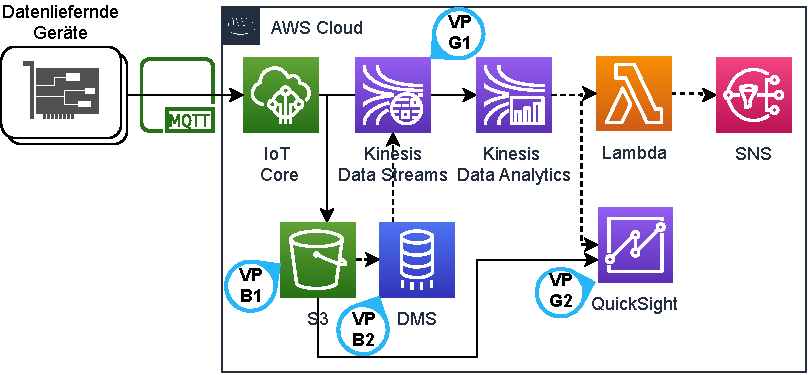
\includegraphics[width=\textwidth]{graphics/Echtzeit-RA-Overview.pdf}
\caption{Top Level View Referenzarchitektur}
\label{abb:TopLevelEchtzeitRA}
\end{figure}

\begin{figure}[H]
\centering
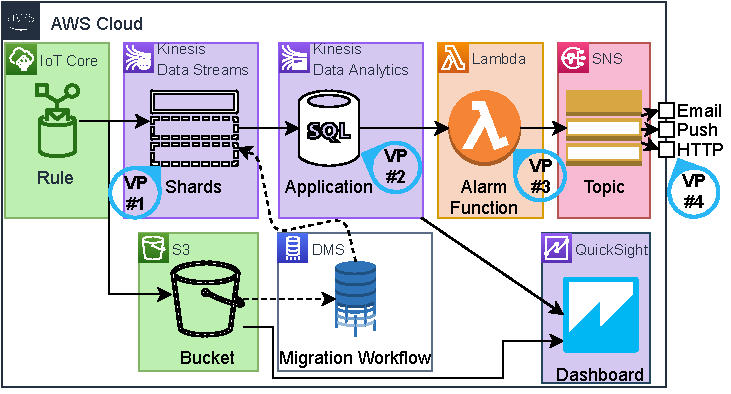
\includegraphics[height=0.33\textheight]{graphics/Echtzeit-RA-Elements.pdf}
\caption{Interagierende Dienstelemente}
\label{abb:ElementeEchtzeitRA}
\end{figure}



\section{Batch Verarbeitung}



\begin{figure}[H]
\centering
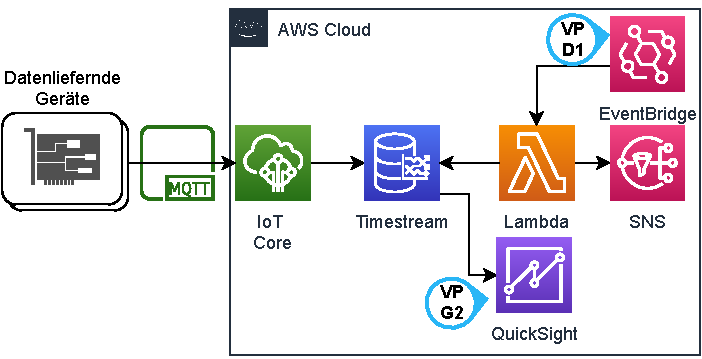
\includegraphics[width=\textwidth]{graphics/DB-RA-Overview.pdf}
\caption{Top Level View Referenzarchitektur}
\label{abb:TopLevelDBRA}
\end{figure}



\begin{figure}[H]
\centering
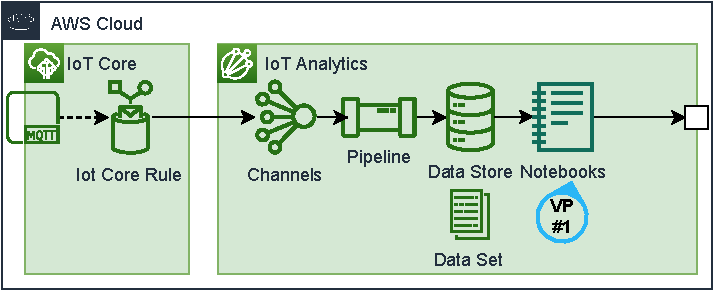
\includegraphics[width=\textwidth]{graphics/DB-RA-Elements.pdf}
\caption{Interagierende Dienstelemente}
\label{abb:ElementeDBRA}
\end{figure}

\section{Einsatzszenarien der Referenzmodelle}